\graphicspath{{introduction/fig/}}

\chapter{Introduction}
\label{chap:introduction}

\section{Background}
In the modern world robots are becoming more and more part of our daily lives and society. For example the Xiaomi house cleaning robot.
Generally in robotics a manipulator (eg.
an arm) is used to manipulate an object in
the environment.

It is easier to bfirst simulate the robots behavior in a
more simple environment which is why we will solve a similar and smaller problem as a step to a complete solution. By doing sp we can save expenses, as it is costly to test a robot in reality while simulation is much cheaper. \newline

The sliding puzzle is a game with a history going back to the 1870's. The aim of the game is to place a shuffled set of 15 numbered tiles into ascending order by sliding and swapping the black/blank tile piece into one of its neighboring tiles. An example of a puzzle being solved is shown in \ref{fig:sliding_puzzle_figs}.

\begin{figure}
	\centering
	\begin{subfigure}{.2\textwidth}
		\centering
		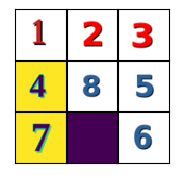
\includegraphics[width=.75\linewidth]{game_states/31.png}
		\caption{1a}
		\label{fig:sfig1}
	\end{subfigure}%
	\begin{subfigure}{.2\textwidth}
		\centering
		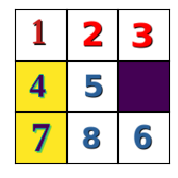
\includegraphics[width=.75\linewidth]{game_states/32.png}
		\caption{1b}
		\label{fig:sfig2}
	\end{subfigure}
	\begin{subfigure}{.2\textwidth}
		\centering
		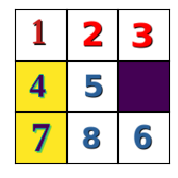
\includegraphics[width=.75\linewidth]{game_states/33.png}
		\caption{1b}
		\label{fig:sfig3}
	\end{subfigure}
	\begin{subfigure}{.2\textwidth}
		\centering
		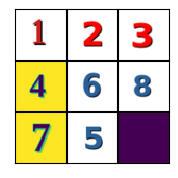
\includegraphics[width=.75\linewidth]{game_states/34.png}
		\caption{1b}
		\label{fig:sfig4}
	\end{subfigure}
	\caption{Figures of a 3x3 sliding puzzle being solved}
	\label{fig:sliding_puzzle_figs}
\end{figure}

\section{Problem Statement/ Research Aim}
In this project
we solve sliding puzzles using
reinforcement learning, where the same algorithm can then later be applied to the robotics problem of moving in an environment. Seen in Figure \ref{fig:sliding_puzzle_figs} is an example 4x4 puzzle.

\section{Project Objectives}
\begin{itemize}
	\item Solve a 2x2 sliding puzzle using Reinforcement learning
	\item Solve a 3x3 puzzle using Reinforcement learning
	\item Puzzles must solve in a reasonable amount of time
\end{itemize}

\section{Scope}
Although there are many methods of solving a problem in RL, in this project we only look at two methods. These are SARSA (State-Action-Reward-State-Action) and Q-learning. 

Typically for problems with large state spaces neural networks are used in conjunction with the Reinforcement Learning techniques, to save computational time. However for this project we used a certain method to overcome the state space limitation which will be discussed later.

\section{Document Outline}
To follow along the report, we first layout the required knowledge in \ref{chap:Literature_Review} for understanding the topics covered in the following chapters. Then next we look at a paper with a similar problem to this reports as well as their solution.

Then in \ref{chap:MDP_and_DP} we describe in detail the mathematical background theory which forms the basis for Reinforcement Learning. In Chapter \ref{chap:RL} we then detail the methods of Reinforcement Learning that will be used to solve our puzzle problem.

Chapter \ref{chap:System_Design} lays out the overarching view of the software system, broken down into functional blocks.
We then in Chapter \ref{chap:Experiments_and_Results} we discuss experiments and results and verify that our solution works. Finally with Chapter \ref{chap:conclusion} the report is concluded.